\cleardoublepage

\newrefsection

\chapter{外文翻译}

\begin{center}
\large\textbf{用于3D生成的原生且紧凑的结构化潜在表示}
\end{center}

\begin{center}
\large\textbf{摘要}
\end{center}


3D生成建模的最新进展已显著提高了生成真实感，
但该领域仍受到现有表示方法的阻碍，
这些方法难以捕捉具有复杂拓扑结构和详细外观的资产。
本文提出了一种从原生3D数据中学习结构化潜在表示的方法，
以应对这一挑战。
其核心是一种新的稀疏体素结构，
称为O-Voxel，
这是一种全方位体素表示，
可编码几何体和外观。
O-Voxel可以稳健地建模任意拓扑结构，
包括开放、非流形和完全封闭的表面，
同时捕获超出纹理颜色的全面表面属性，
例如基于物理的渲染参数。
基于O-Voxel，
我们设计了一种稀疏压缩VAE，
它提供了高空间压缩率和紧凑的潜在空间。
我们使用各种公共3D资产数据集训练包含40亿参数的大规模流匹配模型，
用于3D生成。
尽管规模庞大，
但推理仍然非常高效。
同时，
我们生成的资产的几何形状和材质质量远远超过现有模型。
我们相信我们的方法为3D生成建模提供了显著的进步。

\section{介绍}
近期，
由于潜在3D表示设计方面的创新以及大型潜在学习和生成模型的集成，
3D生成建模取得了前所未有的进展。
这些进步极大地提高了重建保真度和生成真实感，
使3D内容创作更接近实际部署和工业应用。

尽管取得了进展，
但该领域仍然缺乏能够忠实地捕捉任意 3D 资产的完整光谱信息，
并能有效地通过神经网络处理成潜在表示的基本表示方法。
最近的大型 3D 生成模型主要利用等值面场，
（例如，
有符号距离函数）
来表示几何体，
这在处理开放表面、非流形几何体和封闭内部结构方面存在内在局限性。
此外，
大多数现有工作侧重于 3D 形状生成，
而忽略了 3D 资产中固有的外观和材质信息，
这些信息从根本上与形状相关。
有些方法引入了一种结构化的 3D 潜在表示 (SLAT)，
该表示联合建模几何体和外观，
但其对多视图 2D 图像特征输入和纯粹基于渲染的监督的依赖，
导致在捕获复杂结构和材质方面的不足。

在这项工作中，
我们引入了一种新的“无场”稀疏体素结构，
称为O-Voxel。
O-Voxel是一种全方位体素表示，
它编码了几何形状和外观，
充当网格资产和神经网络之间的纽带。
这种结构的“全能性”不仅在于其对几何形状和外观进行建模的综合方法，
还在于其处理它们固有复杂性的强大能力。
对于几何形状，
它可以处理任意拓扑结构，
包括开放、非流形和完全封闭的表面，
这与现有的基于场的方法不同。
通过引入与原始稀疏体素相对应的灵活双重网格结构，
它可以适应复杂的拓扑结构，
而不会造成有损数据预处理，
并保留清晰的边缘特征和法线不连续性，
以实现精确的几何形状再现。
对于外观，
它可以捕获超出单纯纹理颜色的任意表面属性。
在这项工作中，
我们实现了与表面几何形状对齐的基于物理的渲染（PBR）参数，
以实现重新照明功能。
特别是，
它结合了材料不透明度，
使其能够处理半透明表面——这是以前的方法所不具备的功能。

O-Voxel的另一个显著优势是，
它可以与原始3D资产进行即时双向转换。
这些过程既不需要优化，
也不需要渲染。
将网格转换为这种结构仅需在单个CPU上花费几秒钟，
而从中重建表面和材料则在几十毫秒内完成。

鉴于 O-Voxel 表示，
我们设计了一个稀疏 3D 变分自动编码器来学习合适的潜在空间。
从多视图 2D 信息构建的潜在空间相比，
这产生了一个原生的结构化潜在空间。
此外，
我们的目标是建立一个紧凑的潜在空间，
以支持高效和高分辨率的 3D 生成。
利用应用于稀疏体素结构的残差自动编码设计，
我们的 VAE 实现了 16 倍的空间下采样，
这是一个在先前的基于体素的方法中未见的高比率。
我们的方法将具有 1024³ 分辨率的结构压缩为仅约 9.6K 个潜在 tokens，
并在重建时具有可忽略的感知退化。
实验表明，
我们的重建质量大大超过了先前的方法，
尽管使用的 tokens 数量明显更少。
除了实现高分辨率 3D 生成外，
我们紧凑的潜在空间还有助于生成模型的扩展。

我们在学习到的潜在空间中训练大型流匹配生成模型，
用于图像到3D的生成。
这些模型总共包含约40亿个参数，
并在各种公共3D资产数据集上进行训练。
尽管它们规模庞大，
但推理仍然非常高效：
在 NVIDIA H100 GPU 上，
生成 512³ 的完全纹理化资产仅需约 3 秒，
1024³ 分辨率约需 17 秒，
1536³ 分辨率约需 60 秒，
这比现有的大型 3D 生成模型快得多。
同时，
正如我们的实验所证明的，
我们生成的资产的几何和材质质量远远超过现有模型。
我们将公开发布我们所有的模型、代码和数据集，
以方便重现和进一步研究。

\section{相关工作}

\paragraph{用于生成的三维表示}  

有效地表示几何形状和外观以供神经网络处理，
是三维生成中的一个关键挑战。
早期的工作采用隐式场或其离散化结构来表示形状，
例如占据场和有符号距离函数 (SDF) 。
NeRF将几何形状和外观集成到辐射场中，
从而产生逼真的渲染效果，
但存在几何质量低和采样成本高的问题。
非结构化三维表示，包括网格、点云和高斯分布，
提供了显式三维表示，
但缺乏结构规律性，
给网络处理和潜在压缩带来了挑战。
最近的工作引入了为三维生成量身定制的结构化表示。
它们将基于场的等值面建模与稀疏体素相结合，
以实现高分辨率几何。
然而，与我们的方法不同，
它们对基于场的图元的依赖限制了它们表示开放或非流形表面的能力，
并且它们不处理外观。

\paragraph{潜在3D表示}

3D生成领域的最新进展越来越多地从使用显式几何表示转向紧凑的潜在空间，
类似于2D领域中使用的潜在空间。
已经探索了各种潜在公式，包括潜在点云、体素或分层网格和三平面嵌入。
在这些方法中，
两种潜在范式已经成为最近大型3D生成模型的主要选择。
第一种是非结构化潜在空间，
灵感来自 Perceiver 风格的架构，
其中3D数据被编码为无序特征向量。
这些方法可以实现强大的压缩，
但通常受到重建保真度的限制。
第二类是建立在稀疏性先验之上的结构化潜在空间，
这种表示产生高几何精度，
但需要大量的潜在令牌，
从而降低了压缩效率。
一些工作试图通过优化网络计算而不是提高潜在紧凑性来缓解这个问题。
在这项工作中，
我们的方法直接从原生3D输入中学习紧凑的结构化潜在空间，
实现更高的空间下采样率和更少的潜在令牌。

\paragraph{大型3D资产生成模型与系统}
随着大规模3D资产数据集的迅速扩展，
涌现出大量能够生成具有高质量形状和纹理的3D资产的大型模型和系统。
一种常见的范式将生成过程分解为两个阶段：
形状生成和多视角纹理合成。
虽然此流程受益于强大的2D图像扩散骨干网络，
但它通常需要复杂的多视图渲染、烘焙和纹理对齐，
这阻碍了可扩展性，
并且经常引入外观不一致性。
一些方法解决了具有材质信息的3D生成问题，
但仍然依赖于多视图烘焙来合并生成的网格和3D高斯函数以进行资产提取。
相比之下，
我们的方法执行原生的、端到端的3D资产生成，
直接生成高保真、完全纹理化的3D资产，
而无需任何依赖于视角的后处理。

\section{方法}
我们的目标是生成具有任意形状拓扑和灵活材质属性的高分辨率3D资产。
我们的方法概述如图~\ref{fig:approach}所示。
\begin{figure}[htbp]
    \centering
    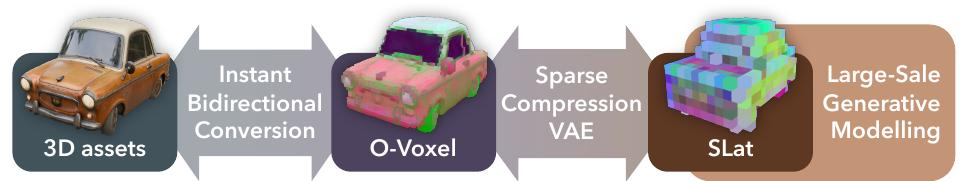
\includegraphics[width=0.8\textwidth]{figure/translation/approach.jpg}
    % 图号和标题
    \caption{方法概述。我们引入O-Voxel用于形状和材质表示（第3.1节），
    在此基础上，我们采用稀疏压缩VAE进行紧凑潜在空间学习（第3.2节），
    并采用大型流模型进行3D生成（第3.3节）。}
    \label{fig:approach}
\end{figure}

\subsection{O-Voxel：一种原生3D表示}
给定一个3D资产，
O-Voxel将其表示为与分辨率为N × N × N的规则3D网格上的稀疏体素相关联的特征元组的集合：
\begin{equation} \label{eq:1}
\bm{f} = \{ (\bm{f}_i^{\text{shape}}, \bm{f}_i^{\text{mat}}, \bm{p}_i) \}_{i=1}^L \tag{1}
\end{equation}

其中
\(\bm{f}_i^{\text{shape}}\) 编码局部几何信息，  
\(\bm{f}_i^{\text{mat}}\) 编码材料属性，  
并且 \(\bm{p}_i \in \{0, 1, \dots, N-1\}^3\) 表示第 \(i\) 个活动体素的坐标。  
与资产不相交的空体素被设置为非活动状态。

\subsubsection{用于形状的灵活双重网格}
由于其灵活的对偶网格公式，
O-Voxel 可以稳健地表示具有任意拓扑的表面，  
在这个对偶网格中，每个原始单元定义一个顶点，
每个原始边定义一个四边形面，  
连接相邻原始单元中的对偶顶点，
通过构建与原始规则体素网格相对应的对偶网格，  
我们的算法灵活地调整对偶顶点的位置和对偶网格面的存在，
以准确表示任意输入表面数据（如图 \ref{fig:convertion} 的第一行所示）

这种表述的灵感来源于对偶轮廓法（Dual Contouring，DC），  
这是一种从带符号网格中提取表面的算法，  
网格的边用埃尔米特数据（即交点和法线）标记，  
最初的DC被设计用于处理离散化的标量场，例如SDF，  
与DC不同，我们不使用任何场表示，  
我们的方法很简单：我们直接使用资产的网格表面来确定边缘相交标志（而不是像DC中那样检测符号变化），  
并分配埃尔米特数据，  
每个与网格相交的边都会激活相应的对偶面，  
然后使用相关的埃尔米特数据来调整对偶顶点的位置，  
给定埃尔米特数据 $\{\bm{q}_i, \bm{n}_i\}$，  
我们使用以下二次误差函数（QEF）以闭合形式计算对偶顶点 $\bm{v}$：

\begin{equation} \label{eq:2}
\min_{\bm{v} \in \text{voxel}}  
e(\bm{v}) =  
\sum_i d^2_{\Pi,i} + \lambda_{\text{bound}} \sum_j d^2_{L,j} + \lambda_{\text{reg}} d^2_{\hat{\bm{q}}} \tag{2}  
\end{equation}

\begin{figure}[htbp]
    \centering
    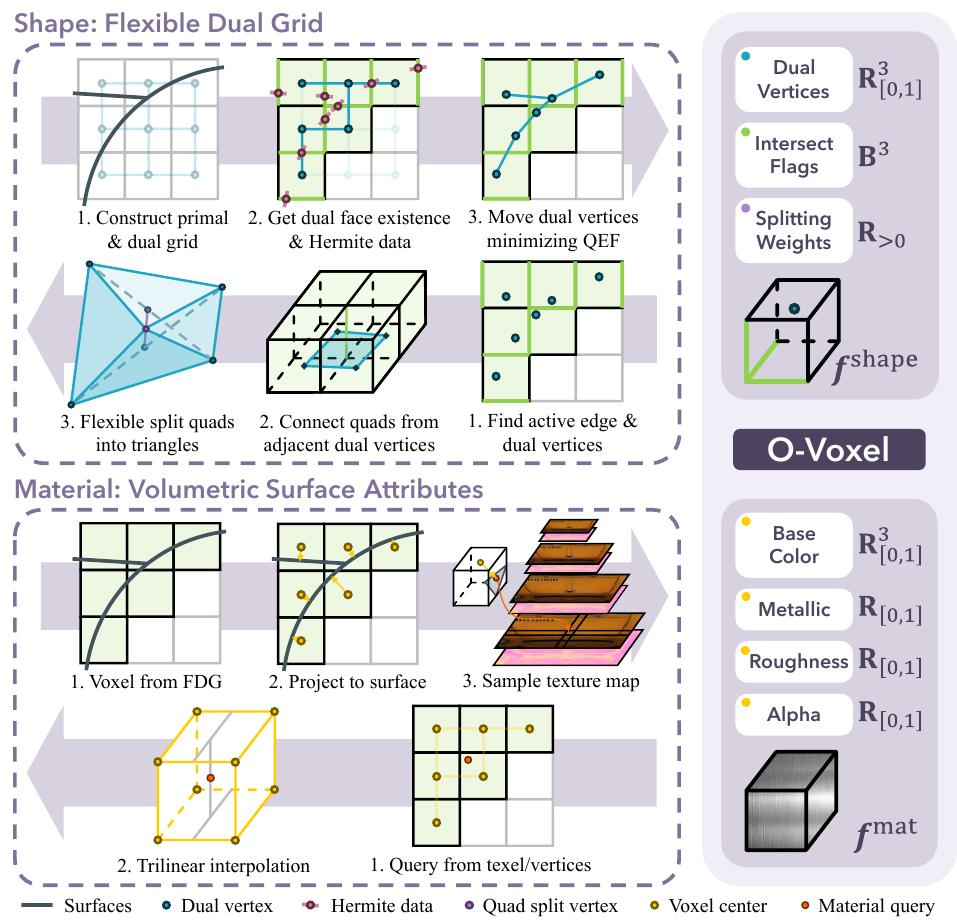
\includegraphics[width=0.8\textwidth]{figure/translation/convertion.jpg}
    % 图号和标题
    \caption{O-Voxel及其在3D资产和O-Voxel之间的即时双向转换的示意图}
    \label{fig:convertion}
\end{figure}

原始的直流QEF仅包含第一个分量，该分量衡量了  
$\bm{v}$  
到由 $\{\bm{q}_i, \bm{n}_i\}$ 确定的平面的平方距离，  
$d^2_{\Pi,i} = (\bm{n}_i \cdot (\bm{v} - \bm{q}_i))^2$，  
我们引入了一个额外的误差项，该误差项惩罚了  
$\bm{v}$  
与网格的任何与原始单元相交的边界边之间的距离，  
$d^2_{L,j} = \| (\bm{v} - \bm{o}_j) - ((\bm{v} - \bm{o}_j) \cdot \bm{d}_j)\bm{d}_j \|^2$，  
以及一个正则化项，该正则化项鼓励  
$\bm{v}$  
保持接近相交点的平均值，  
$d^2_{\hat{\bm{q}}} = \| \bm{v} - \bar{\bm{q}} \|^2$，  
前者引导对偶顶点与边界边对齐，从而改善开放表面的表示，而后者则鼓励更平滑的顶点分布并稳定QEF优化以防止奇异性。

基于上述算法描述，对于每个活跃体素，我们的几何特征  
$\bm{f}^{\text{shape}}_i$  
包括：
\begin{itemize}
\item \textbf{对偶顶点} $\bm{v}_i \in \mathbb{R}^3 [0,1]$，网格内的一个顶点，用于表示局部表面形状，
\item \textbf{边缘相交标志} $\bm{\delta}_i \in \{0,1\}^3$，它确定相邻对偶顶点之间的四边形连接，我们分别使用沿 $\bm{X}$、$\bm{Y}$ 和 $\bm{Z}$ 轴的 3 个预定义体素边上的表面-边相交（例如，那些共享最小坐标角的边），
\item \textbf{拆分权重} $\bm{\gamma}_i \in \mathbb{R}_{>0}$，控制四边形面自适应细分为三角形的方式，遵循[53]中灵活的拓扑规则，
\end{itemize}

\paragraph{网格 → O-Voxel}
给定一个网格，我们首先识别与网格表面相交的所有体素边缘，
并将它们的相邻体素标记为激活状态，  
交点及其法线是从网格三角形解析计算得到的，从而产生埃尔米特数据，  
然后通过求解公式 (\ref{eq:2}) 中的 QEF 来计算每个激活体素的对偶顶点 $\bm{v}$。

\paragraph{O-Voxel → 网格}
从一个O-体素，我们通过连接相交边上的对偶顶点来恢复网格表面，
从而在相邻的活动体素之间形成四边形面。
每个四边形可以根据分割权重自适应地细分为两个三角形，
从而使表面更好地符合局部几何特征。

灵活双网格具有以下几个\textbf{关键优势}：
\begin{enumerate}
\item \textbf{瞬时双向转换}——它能够实现与网格的快速映射，并支持以最小的计算开销进行高分辨率转换，  
先前工作中代价高昂的流程，如 SDF 评估、floodfill 过程和迭代优化，都不再需要，
\item \textbf{可耕性-拓扑建模}——它不受水密性和流形约束的限制，从而能够稳健地处理任意几何形状，包括自相交表面和完全封闭的内部结构，
\item \textbf{高精度和锐利特征保持}——通过算法设计，对偶顶点 $\bm{v}$ 与局部几何特征对齐[25]，从而保持锐利特征，  
此外，对偶顶点位置和分裂权重 $\bm{\gamma}_i$ 可以通过神经网络接收可学习的调整，使用其他监督信息，例如渲染损失（见第 ~\ref{sec:render_loss} 节），进一步增强了几何体的灵活性和精度，
\end{enumerate}

\subsubsection{用于材质的体积属性}
O-Voxel可以对齐表面几何结构的任意表面属性进行建模，包括颜色和其他材质属性，  
在这项工作中，我们实现了基于物理的渲染 (PBR) 参数，以捕捉材料固有的光-表面相互作用特性，  
具体来说，我们每个激活体素的材质特征 $\bm{f}^{\text{mat}}_i$ 由六个通道组成：

\begin{equation}
    \bm{f}^{\text{mat}}_i = (\bm{c}_i, m_i, r_i, \alpha_i) \tag{3}
\end{equation}

其中 $\bm{c}_i \in \mathbb{R}^3 [0,1]$ 表示基色，  
$\bm{m}_i \in [0,1]$ 表示金属比例，  
$\bm{r}_i \in [0,1]$ 表示粗糙度，  
$\bm{\alpha}_i \in [0,1]$ 表示不透明度，  
这种参数化遵循现代基于物理的渲染流程中广泛采用的标准 PBR 约定，  
如图~3 所示，O-Voxel数据和网格纹理之间的转换简单而快速。

\paragraph{纹理 → O-Voxel}
对于一个激活的体素，我们将其中心投影到每个相交的三角形上，
并使用UV坐标和适当的mipmap级别从纹理贴图中采样每个材质属性。
采样的属性基于点到表面的距离进行加权平均，
以获得最终值。有关此过程的更多详细信息，请参见补充材料。

\paragraph{O-Voxel → 纹理}
在重建过程中，对于每个查询点——无论是用于顶点着色的网格顶点位置，
还是对应于纹理贴图纹素的3D表面点——材料属性都是通过相邻体素属性的三线性插值获得的。
重建后的网格即可用于渲染，无需任何额外的后处理。

\subsection{稀疏压缩VAE}
我们应用 VAE 从 O-Voxel 数据中学习合适的潜在空间，  
我们的目标是获得一个紧凑的潜在空间，以促进高效、高分辨率的 3D 生成，  
我们设计了一个稀疏压缩 VAE (SC-VAE) 来实现这一点。

\subsubsection{网络架构}

我们的 SC-VAE 的架构如图 \ref{fig:structure} 所示，  
与先前工作中基于 Transformer 的设计不同，我们的 SC-VAE 采用完全稀疏卷积网络，
该网络在高分辨率下具有计算效率，并且可以很好地跨尺度泛化，  
遵循 U 形 VAE 设计，我们的编码器通过多个残差块分层下采样稀疏体素特征，
解码器镜像此过程以进行重建，  
我们精心设计了残差和（下/上）采样块，以实现高压缩编码和忠实恢复。

\begin{figure}[htbp]
    \centering
    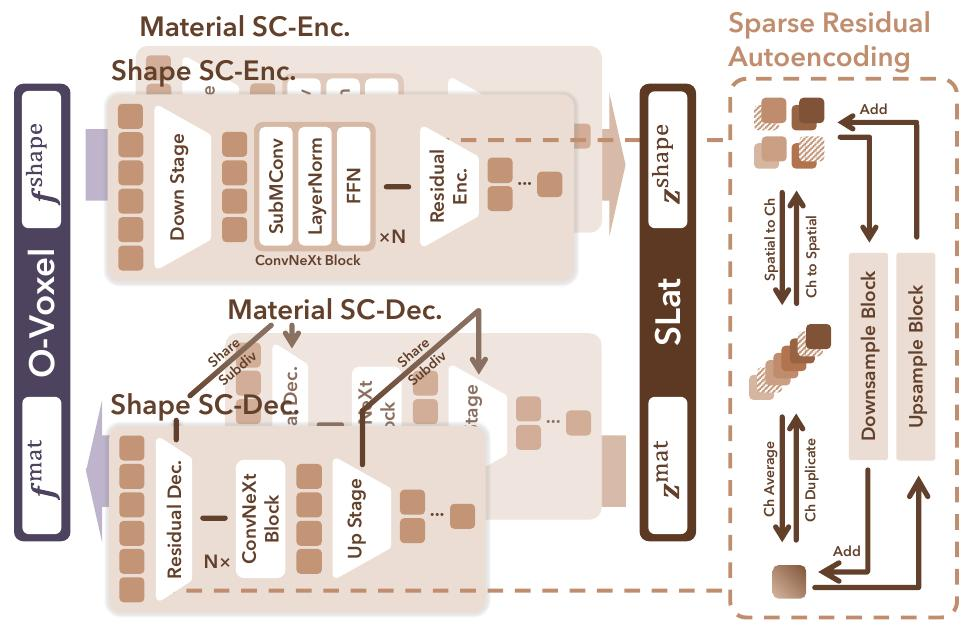
\includegraphics[width=0.8\textwidth]{figure/translation/structure.jpg}
    % 图号和标题
    \caption{SC-VAE 的网络结构}
    \label{fig:structure}
\end{figure}

\paragraph{稀疏残差自编码层}
我们将 DC-AE 中的残差自编码原理应用于稀疏体素数据，  
通过在下采样和上采样块中引入非参数残差捷径来实现，  
这些捷径通过在稀疏网格中重新排列空间和通道维度之间的信息，  
缓解了高空间压缩下的优化挑战。

具体而言，对于 2 的下采样因子，我们将每个体素的八个子体素聚合到其通道维度中，  
给定输入特征 $F_{\text{fine}} \in \mathbb{R}^C$ 和目标粗糙特征 $F_{\text{coarse}} \in \mathbb{R}^{C'}$（通常 $C' = 2C$），  
我们有：
\begin{equation}
\begin{split}
F^{\text{raw}}_{\text{coarse}} &= \text{stack}\left(F_{\text{child}1}, \dots, F_{\text{child}8}\right) \in \mathbb{R}^{8C}, \\
F_{\text{coarse}} &= \text{avg\_groups}\left(F^{\text{raw}}_{\text{coarse}}\right) \in \mathbb{R}^{C'}.
\end{split}
\tag{4}
\end{equation}
其中，avg groups 操作对分组通道求平均值，
以产生粗略的残差估计。由于稀疏性，缺失的体素贡献零向量。

在上采样过程中，对称的通道到空间快捷方式将每个粗略特征分配回其邻域：
\begin{equation}
\begin{split}
F^{\text{raw}}_{\text{fine}} &= \text{unstack}\left(F_{\text{coarse}}\right) \in \mathbb{R}^{8C'/8}, \\
F_{\text{fine}} &= \text{dup\_groups}\left(F^{\text{raw}}_{\text{fine}}\right) \in \mathbb{R}^{C}.
\end{split}
\tag{5}
\end{equation}
其中，dup 将每个组内的副本通道分组，以匹配目标维度。

\paragraph{早期剪枝上采样器}
为了进一步提高效率，我们为上采样器采用了一种早期剪枝机制 [51]，  
在每个上采样步骤之前，该模块预测一个二元掩码 $\hat{\rho} \in \{0,1\}^8$，用于指定每个父节点的活动子体素，  
随后跳过非活动节点，从而大大降低运行时间和内存成本。

\paragraph{优化残差块}
稀疏卷积在高稀疏度数据下表现出较低的有效计算和参数效率。
鉴于此，我们通过减少卷积层并结合逐点MLP来重新设计残差块，
以实现更丰富的特征转换。
具体来说，我们用单个卷积层和更少的归一化及激活层来代替两个卷积层的标准设计，
遵循ConvNeXt风格的简化。
第二个卷积被一个宽的逐点MLP所取代——类似于Transformer FFN——它扩展了通道维度，
以增强非线性和表示能力。如我们的实验所示，这种修改不影响效率，但提高了重建质量。

\subsubsection{VAE 训练} \label{sec:render_loss}
SC-VAE 的训练分为两个阶段，  
在第一阶段，我们使用低分辨率数据，通过直接的 O-Voxel 重建损失和 KL 损失，快速稳定学习，  
对于几何特征，均方误差（MSE）和二元交叉熵（BCE）损失分别应用于对偶顶点位置 $\bm{v}$ 和对偶面片标志 $\bm{\delta}$，  
材质属性 $\bm{f}^{\text{mat}}$ 和剪枝掩码 $\bm{\rho}$ 分别由 L1 损失和 BCE 损失监督：
\begin{equation}
\begin{split}
\mathcal{L}_{s1} &= \lambda_v \|\hat{v} - v\|_2^2 + \lambda_\delta \, \text{BCE}(\hat{\delta}, \delta) \\
&\quad + \lambda_\rho \, \text{BCE}(\hat{\rho}, \rho) + \lambda_{\text{mat}} \|\hat{f}^{\text{mat}} - f^{\text{mat}}\|_1 + \lambda_{\text{KL}} \mathcal{L}_{\text{KL}}
\end{split}
\tag{6}
\end{equation}

在第二阶段，我们添加了基于渲染的高分辨率感知监督，以增强几何和材质的逼真度，  
我们渲染了掩模、深度和法线贴图，并使用 L1 损失对其进行监督，并在法线上增加了 SSIM 和 LPIPS 项，  
材质属性也通过这些感知损失进行渲染和监督，  
损失可以写成：
\begin{equation}
\mathcal{L}_{s2} = \mathcal{L}_{s1} + \mathcal{L}_{\text{render}}.
\tag{6}
\end{equation}
我们随机地在周围放置具有浅近平面的相机，
以切片穿过表面，从而鼓励模型捕获外部和内部结构。
损失的更多细节在补充材料中提供。

为了便于形状和材质的顺序生成方案（特别是，为了能够对给定的形状应用材质生成），
我们使用两个SC-VAE学习解耦的潜在空间：一个对形状进行建模，
而另一个对以形状VAE在上采样期间的细分结构为条件的材质进行建模。

\subsection{生成建模}
基于学习到的潜在空间，我们构建了一个可扩展的生成框架，
遵循的总体设计。我们采用了基于完整DiT的架构，
并使用流匹配范式进行训练，并扩展了的流程，
以充分利用我们新的潜在变量的能力。

\paragraph{模型和生成流程}
完整的生成过程分为三个阶段，涉及三个模型：
1) 稀疏结构生成，预测稀疏体素网格的占用布局；
2) 几何体生成，在活动体素内生成几何体潜在变量；
3) 材质生成，合成与几何体结构对齐的材质潜在变量。
前两个阶段主要遵循[65]的策略，形成资产的几何骨干。
新颖的材质生成阶段直接在原生3D空间中对PBR材质进行建模。
一个稀疏的DiT预测材质潜在变量，该变量以输入图像和生成的几何体潜在变量为条件。
这种设计将几何体和材质生成统一在相同的原生3D潜在域中，并确保它们在任意拓扑下空间对齐。


\paragraph{架构和训练细节}
我们所有的DiT模块都采用AdaLN-single调制和旋转位置嵌入(RoPE)，
以获得更好的可扩展性和跨分辨率泛化能力。
图像条件特征提取自DINOv3-L。
受益于SC-VAE实现的高空间压缩，我们的稀疏DiT丢弃了
中的卷积打包和跳跃连接设计，从而产生了一种vanilla风格的DiT，
降低了复杂性并提高了效率。

我们首先使用 $512 \times 512$ 的条件图像训练稀疏结构生成，以学习粗略的占据先验并建立全局稀疏布局，  
在随后的阶段中，训练以渐进的方式进行，逐步提高空间和视觉分辨率，  
几何体和材质生成器从 $512^3$ 输出（$32^3$ 潜在分辨率）扩展到 $1024^3$ 输出（$64^3$ 潜在分辨率），条件图像分辨率相应地提高到 1024，  
这种渐进式策略允许学习到的先验在不同分辨率之间平滑转移，从而能够高效地训练大规模稀疏 DiT，同时保持几何体和材质的逼真度。

\section{实验}

\paragraph{实现细节}
我们的 SC-VAE 在过滤掉没有 PBR 材质的资产后，
使用 Trellis-500K 设置进行训练，
从而得到来自 Objaverse-XL、ABO 和 HSSD 的精选集合。
我们使用优化的 Triton 实现来进行子流形卷积 ，以进一步提高训练速度。
SC-VAE 在 16 个 H100 GPU 上进行训练，批量大小为 128。

生成模型在一个扩展的约 80 万个资产的集合上进行训练，并使用 TexVerse [77] 进行增强，以丰富 PBR 的多样性和真实感，  
对于图像提示，我们在 Blender [10] 中为每个资产渲染 16 个视图，并随机化 FoV 和光照，  
所有模型都使用 AdamW [38]（学习率 $1 \times 10^{-4}$，权重衰减 $0.01$）和无分类器引导（dropout 率 0.1）进行训练，  
我们框架中的每个 DiT 包含大约 13 亿个参数（宽度：1536，块：30，头：12，MLP 宽度：8192），在 32 个 H100 GPU 上以 256 的批量大小进行训练。

对于重建评估，我们使用 Toys4K 基准以及一个精选的测试集，
该测试集包含 90 个资产，这些资产具有复杂的 PBR 材质和来自最近 Sketchfab 资产的详细形状，
这些资产是在过去两年内发布的，  
这两个测试集在训练期间都是未见过的，  
对于生成质量比较和用户研究，使用 100 个 AI 生成的图像提示，以确保训练与测试的不相交性，  
来自 nvdiffrec 的拆分求和渲染器用于 PBR 资产渲染，  
所有运行时统计数据均在 NVIDIA A100 GPU 上报告，  
其他详细信息在补充材料中提供。

\subsection{3D资产重建}

\paragraph{形状重建}
我们与四个具有代表性的基线方法进行比较：基于 Shape2Vecset 的 Dora，一种基于稀疏体素结构的 TRELLIS，Direct3D-s2，以及 SparseFlex，  
为了评估，我们采用了多种指标：  
（i）网格距离（MD），计算为双向点到网格距离，并使用 F1 分数来衡量包括内部结构的网格重建保真度，  
（ii）倒角距离，使用 F1 分数计算从可见表面采样的点云，仅关注外部形状，  
（iii）使用渲染法线贴图的 PSNR 和 LPIPS 的表面质量指标。

如表\ref{table:comparison} 所示，尽管仅使用了适量的 tokens，并且运行时间明显更少，但我们的方法在所有指标上始终大幅优于所有基线，  
这不仅证明了其卓越的几何保真度、更精细的细节保留以及更准确的内部结构建模，  
还证明了我们方法的高效率。
\begin{table}[t]  % t表示顶部，h=here，b=底部
    \centering
    \caption{形状重建效率和保真度的比较。MD和CD以[NT0]×106报告；运行时间在A100 GPU上测量。}
    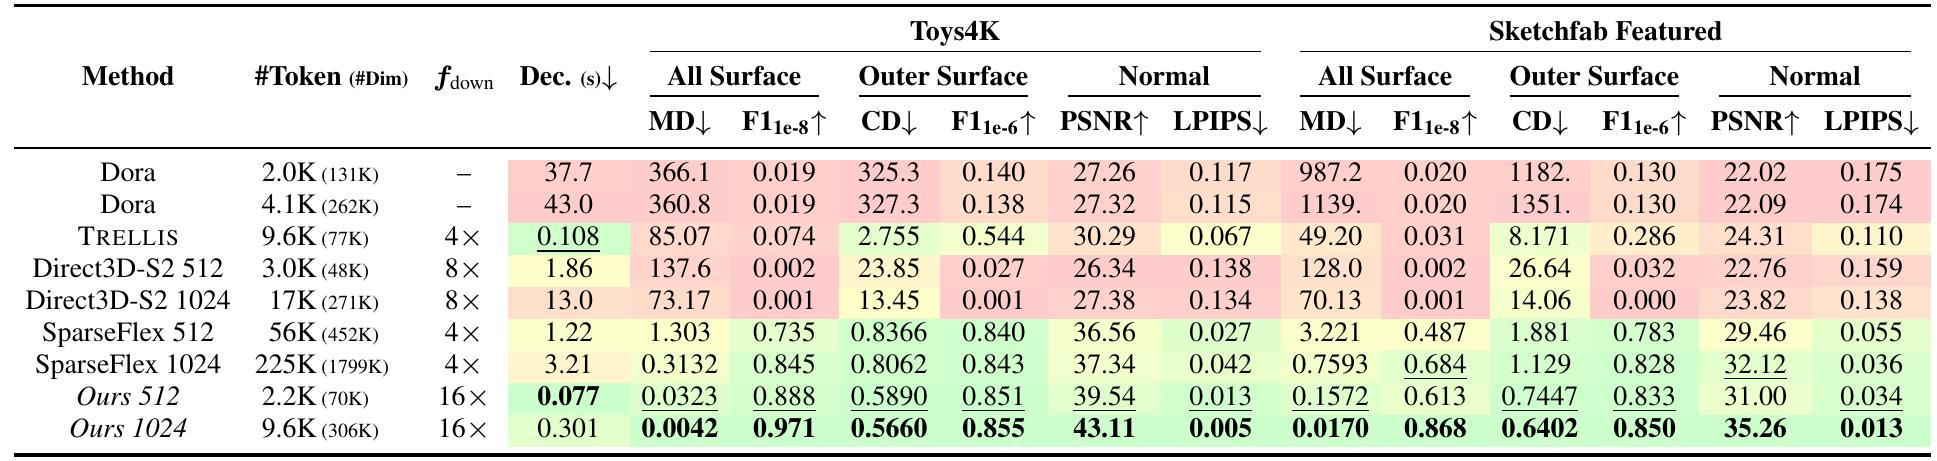
\includegraphics[width=0.8\textwidth]{figure/translation/comparison.jpg} 
    \label{table:comparison} % 用于引用
\end{table}

\paragraph{材质重建}
由于没有合适的基线仅用于编码给定形状的材质属性，我们仅报告我们方法的指标，  
我们使用 PSNR 和 LPIPS 评估直接渲染的 PBR 属性贴图和着色图像的保真度，  
我们的方法在 PBR 属性上达到 $38.89\,\mathrm{dB} / 0.033$，在着色图像上达到 $38.69\,\mathrm{dB} / 0.026$，  
证明了忠实的材质再现和一致的几何体-外观对齐。

\subsection{图像到3D生成}
接下来，我们通过生成以输入图像为条件的3D资产来评估我们框架的生成能力。
图 \ref{fig:high-quality} 给出了代表性的结果，展示了几何保真度和材质的真实感。
\begin{figure}[htbp]
    \centering
    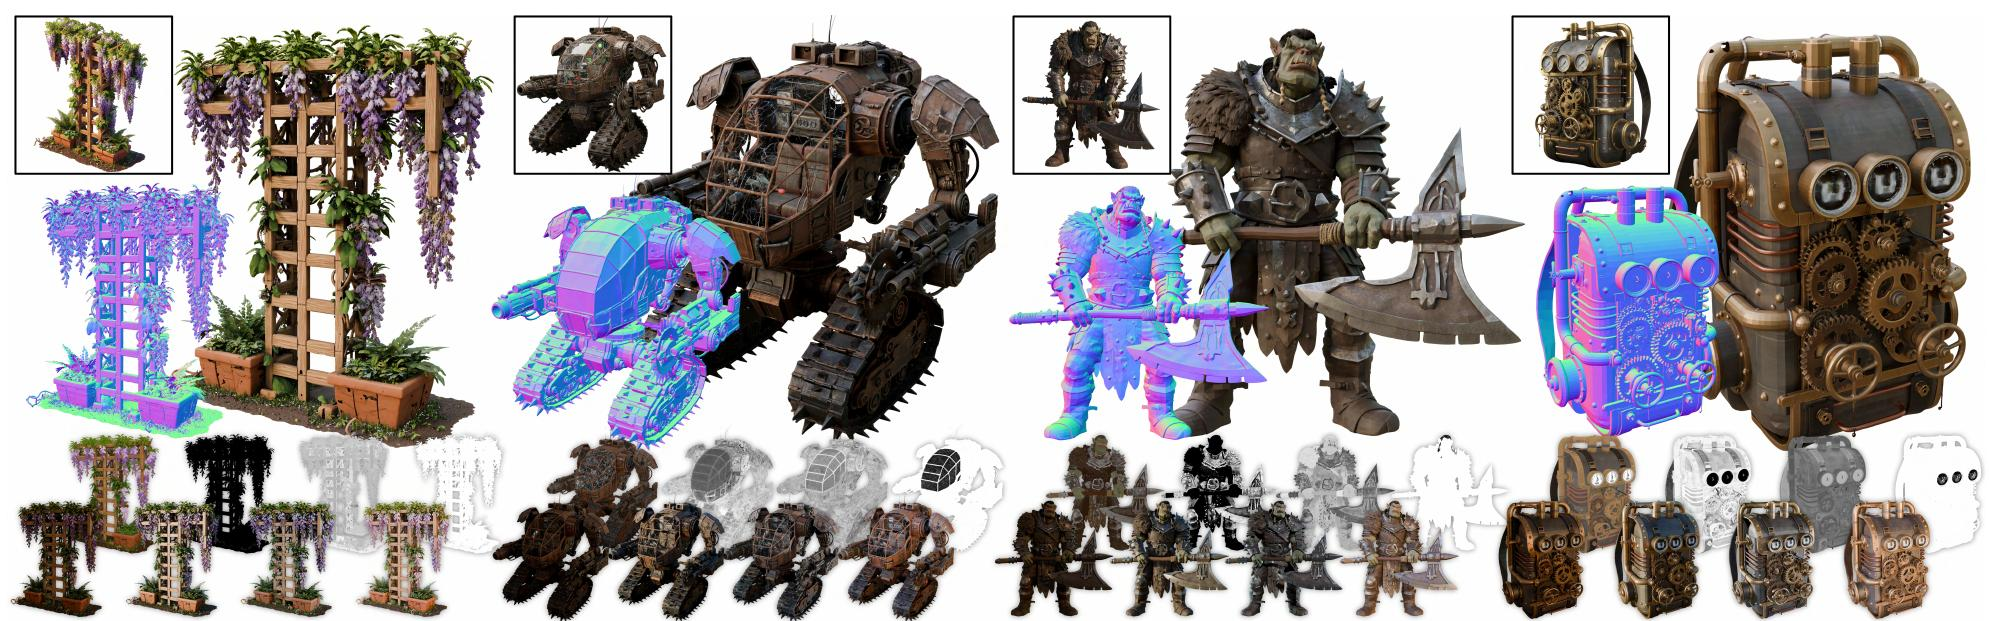
\includegraphics[width=0.8\textwidth]{figure/translation/high-quality.jpg}
    % 图号和标题
    \caption{由我们的方法生成的高质量3D资产，具有复杂的几何细节和物理上精确的材料，
    并具有很高的视觉保真度，包括薄结构、开放表面和半透明区域，这些都突出了模型的表达能力。}
    \label{fig:high-quality}
\end{figure}

我们的方法利用压缩 O-Voxel 的紧凑潜在空间，  
生成的资产能够忠实地保留精细结构、锐利的表面特征以及内部复杂或非流形形状——范围从精细的齿轮、
封闭的驾驶舱到开放的树叶和花朵，  
它还能重现生动、逼真的 PBR 纹理，并在新的光照条件下呈现物理上一致的着色，
包括具有挑战性的半透明或反射材料，如玻璃和金属，  
总而言之，这些结果表明，我们的原生 3D 潜在空间能够生成紧密对齐、
高保真度的几何体和照片般真实的视觉效果，即使对于拓扑结构复杂的资产也是如此。

\paragraph{定性比较}
我们将我们的方法与最先进的3D生成系统进行比较，
包括TRELLIS 、Hi3DGen、Direct3D-s2 、Step1X3D 和
Hunyuan3D 2.1。图 \ref{fig:visual} 中的样本表明，
我们的方法实现了卓越的生成质量——提供准确而细致的几何形状、
物理上合理的材质以及忠实的提示对齐。

\begin{figure}[htbp]
    \centering
    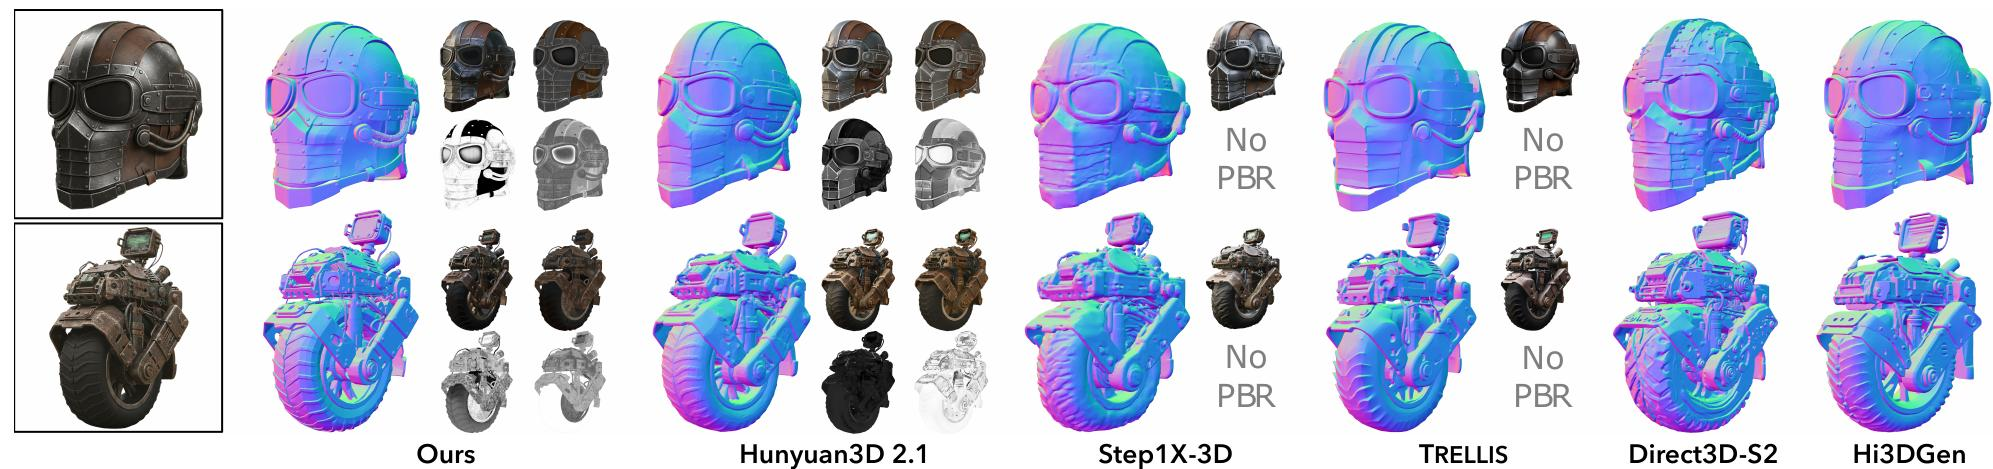
\includegraphics[width=0.8\textwidth]{figure/translation/visual.jpg}
    % 图号和标题
    \caption{由我们的方法生成的高质量3D资产，具有复杂的几何细节和物理上精确的材料，
    并具有很高的视觉保真度，包括薄结构、开放表面和半透明区域，这些都突出了模型的表达能力。}
    \label{fig:visual}
\end{figure}

\paragraph{定量比较}
我们使用人工智能生成的图像进行定量评估，  
视觉对齐使用 CLIP 分数进行测量，而多模态模型 ULIP-2 和 Uni3D 用于评估几何相似性，  
表\ref{table:metric} 显示，我们的方法在所有指标上都获得了最高的对齐分数，  
表明在视觉和几何一致性方面具有明显的优势。

\begin{table}[t]  % t表示顶部，h=here，b=底部
    \centering
    \caption{图像到3D生成结果的比较。-N：使用法线贴图测量。}
    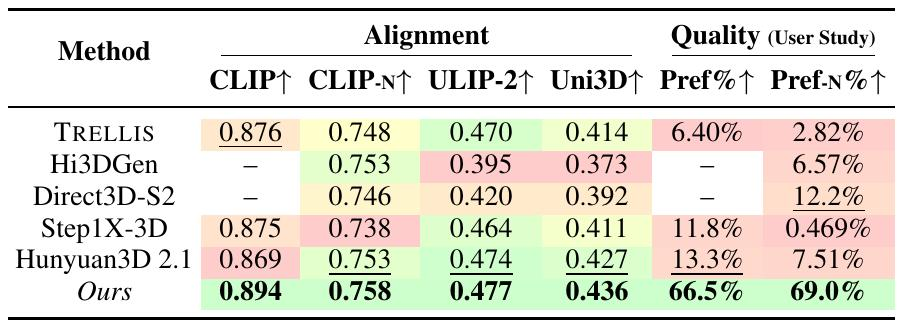
\includegraphics[width=0.8\textwidth]{figure/translation/metric.jpg} 
    \label{table:metric} % 用于引用
\end{table}

我们还进行了约 40 名参与者的用户研究，以评估感知质量，  
使用 100 个 AI 生成的图像提示，我们在相同的条件下使用每种方法生成资产，不进行筛选，并收集偏好投票，  
表 \ref{table:metric} 显示我们的方法受到参与者的青睐，  
突出了其在视觉真实感、几何细节的丰富性以及与输入提示的对齐方面明显的优势。

\subsection{形状条件纹理生成}
我们生成流程的第三阶段可以独立用作 3D PBR 纹理合成模型，给定 3D 网格和参考图像，  
为了评估其性能，我们与具有代表性的基线方法进行比较：
多视角 PBR 生成和融合方法 Hunyuan3D-Paint，以及基于 UV 的 TEXGen。

如图\ref{fig:pbr}所示，多视图方法通常会受到形状和合成图像之间以及不同视图之间不一致性的影响，  
从而导致重影或纹理模糊，  
基于 UV 的方法会受到模糊的 UV 图表和接缝伪影的影响，从而导致视觉质量下降，  
相比之下，我们的框架在 3D 中自然地执行外观推理，  
这可以实现更清晰的纹理、一致的形状-材质对齐，以及内部表面的纹理合成，  
这对于具有遮挡或非流形几何体的复杂资产至关重要。

\subsection{消融和设计分析}
我们进行消融研究，以分析 SC-VAE 的架构设计，  
所有消融实验均在分辨率为 $256^3$ 的精选 Sketchfab 资产上进行。

\paragraph{稀疏残差自编码}
为了评估稀疏残差自编码层的效果，我们将 SC-VAE 与使用平均池化和最近邻上采样的基线进行比较，  
如表\ref{table:ablation} 所示，基线表现出严重的质量下降：MD 增加了 69\%，  
并且在 16 倍压缩时，PSNR 降低 0.5\,dB，  
在 32 倍压缩时恶化至 526\% 和 1.6\,dB，  
相比之下，稀疏残差设计在各种压缩比下保持了高保真度，  
证实了其在强空间瓶颈下的鲁棒性。
\begin{figure}[htbp]
    \centering
    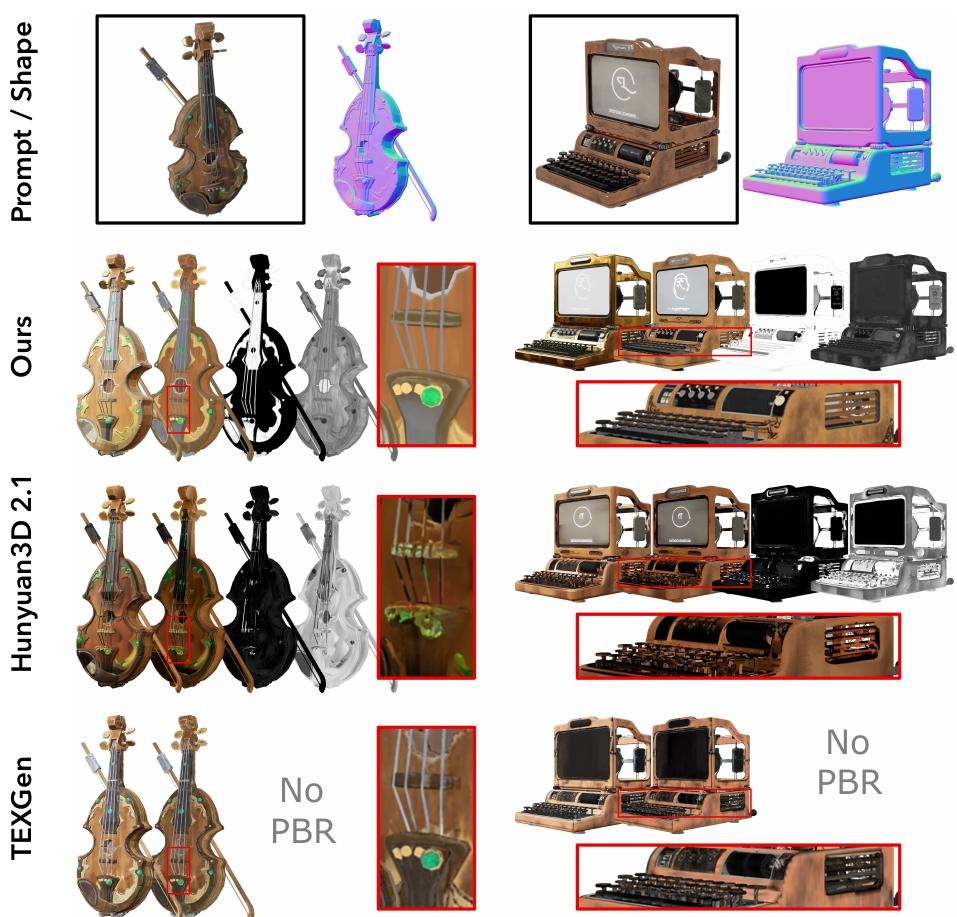
\includegraphics[width=0.8\textwidth]{figure/translation/PBR.jpg}
    % 图号和标题
    \caption{ PBR 纹理生成的可视化比较}
    \label{fig:pbr}
\end{figure}
\begin{table}[t]  % t表示顶部，h=here，b=底部
    \centering
    \caption{SC-VAE 架构设计的消融研究}
    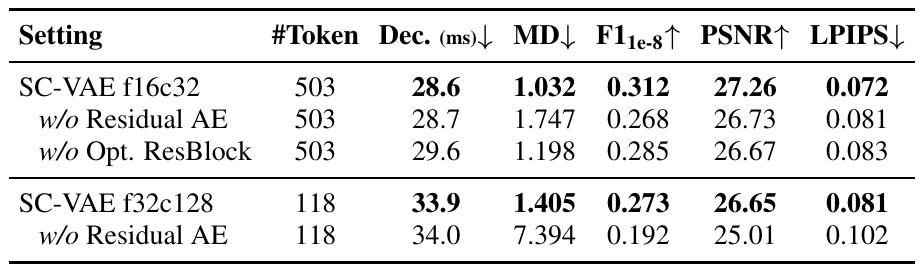
\includegraphics[width=0.8\textwidth]{figure/translation/ablation.jpg} 
    \label{table:ablation} % 用于引用
\end{table}

\paragraph{优化残差块}
为了评估优化残差块的效果，我们将 SC-VAE 与使用标准残差块的基线进行比较，  
表~3 显示，这导致重建质量明显下降：MD 增加 16\%，PSNR 降低 0.6\,dB，而运行时间保持不变，  
这证实了混合稀疏卷积和逐点 MLP 设计能够更好地保留精细尺度细节，而不会牺牲效率。

\subsection{测试时计算和分辨率缩放}
我们的框架能够灵活地在测试时调整计算量和分辨率，这得益于我们紧凑潜在空间的效率，  
值得注意的是，由于 SC-VAE 的 16 倍空间压缩，我们的生成过程所需的 tokens 明显少于先前的方法，  
这种效率允许第二阶段生成器的级联应用，从而能够高效地合成分辨率超过训练规模的形状，  
具体来说，在从几何潜在空间预测 O-Voxel 结构后，我们可以将其下采样为更高分辨率的稀疏结构布局
（例如，将生成的 $1024^3$ O-Voxel 最大池化为 $96^3$ 稀疏结构分辨率），  
随后，我们重新应用几何生成阶段以获得更高分辨率的形状（将 $96^3$ 稀疏结构转换为 $1536^3$ O-Voxel），  
参见图\ref{fig:testing}（左）的示例。
\begin{figure}[htbp]
    \centering
    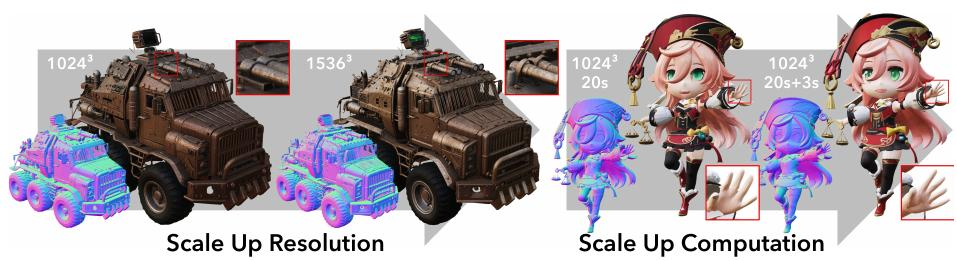
\includegraphics[width=0.8\textwidth]{figure/translation/testing.jpg}
    % 图号和标题
    \caption{在测试时，提高分辨率以获得更精细的细节，并提高计算能力以获得更高的质量。（最好放大观看）}
    \label{fig:testing}
\end{figure}

在训练分辨率范围内操作时，可以应用类似的策略来提高生成质量，  
与其直接使用第一阶段生成的稀疏结构，不如通过对生成的 O-Voxel 进行降采样来获得替代方案
（例如，将 $512^3$ O-Voxel 降采样到 $64^3$ 稀疏结构），  
这可以纠正局部错误，并为后续的高分辨率生成产生更清晰的布局（例如，$1024^3$ O-Voxel），  
这种级联推理机制在计算效率和生成质量之间提供了可控的权衡，  
如图\ref{fig:testing}（右）所示，级联推理产生了更精细的细节并增强了结构稳定性。

\section{结论}
我们提出了一种学习全面而紧凑的结构化 3D 潜在表示的方法，用于 3D 生成，  
一项关键创新是 O-Voxel，一种能够编码复杂几何体和材料的全方位体素表示，  
我们还引入了一种稀疏压缩 VAE，它在 O-Voxel 上实现了高空间压缩率，从而构建潜在空间，  
与现有方法相比，我们的大型流匹配模型在保持高效率的同时，提供了明显更优越的生成质量，  
我们相信我们的方法在 3D 生成建模方面提供了一个显著的进步，  
提高了 3D 内容创建的效率和真实感，并为跨各种领域的更广泛应用开辟了道路。


% 参考~\cite{xiang2025native}
% \begingroup
%     \linespreadsingle{}
%     \printbibliography[title={外文翻译参考文献}]
% \endgroup
